%% HyperVul: IEEE Conference Paper
%% Compile on Overleaf with: pdfLaTeX, then BibTeX, then pdfLaTeX x2
%% Document class: IEEEtran conference

\documentclass[conference]{IEEEtran}
\IEEEoverridecommandlockouts

\usepackage{cite}
\usepackage{amsmath,amssymb,amsfonts}
\usepackage{algorithmic}
\usepackage{graphicx}
\usepackage{textcomp}
\usepackage{xcolor}
\usepackage{booktabs}
\usepackage{multirow}
\usepackage{array}
\usepackage{tikz}
\usetikzlibrary{shapes.geometric, arrows.meta, positioning, fit, backgrounds, calc}
\usepackage{listings}
\usepackage{url}

% --- Listing style for Solidity snippets ---
\lstdefinestyle{solidity}{
  basicstyle=\ttfamily\scriptsize,
  keywordstyle=\color{blue!70!black}\bfseries,
  commentstyle=\color{gray},
  numberstyle=\tiny\color{gray},
  numbers=left,
  numbersep=4pt,
  breaklines=true,
  frame=single,
  framesep=3pt,
  xleftmargin=10pt,
  morekeywords={function,public,external,payable,require,address,uint,mapping,call,if}
}

% --- Convenience macros ---
\newcommand{\hypervul}{\textsc{HyperVul}}
\newcommand{\hyperedgenn}{\textsc{HyperedgeNN}}
\newcommand{\pmstd}[2]{$#1 \pm #2$}

\begin{document}

\title{\hypervul{}: Vulnerability Detection via Higher-Order\\
Interaction Hyperedges in Solidity Smart Contracts}

\author{
\IEEEauthorblockN{Anonymous Author(s)}
\IEEEauthorblockA{\textit{Affiliation}\\
\textit{Institution}\\
City, Country \\
email@domain.edu}
}

\maketitle

\begin{abstract}
Smart contracts manage billions of dollars of on-chain value and are immutable once
deployed, making automated vulnerability detection a critical safeguard. Existing
machine-learning detectors operate either at the function level or over pairwise
program graphs (AST, CFG, DFG, or call graphs). Both families decompose the
multi-entity interaction patterns that are the true locus of many vulnerabilities:
a reentrancy bug, for example, arises from the \emph{joint} presence of a function,
an accessed state variable, an external call, and a missing guard. Pairwise edges
fragment this $n$-ary relation into isolated binary signals. We propose \hypervul{},
which models each vulnerability-relevant interaction as a \emph{typed hyperedge} over
\{function, state variables, external callees, guard signals, cross-contract context\}
and classifies it without decomposition. \hypervul{} contributes (i) an
interaction-level hyperedge representation, (ii) security-aware symbolic feature
augmentation, and (iii) interaction-level localization of supporting evidence. Under
a controlled three-question evaluation across five random seeds, \hypervul{}
outperforms seven generic baselines on F1, F2, and PR-AUC; a representation ablation
holding the candidate interactions fixed shows that the hyperedge encoding
consistently beats set-pooling and pairwise GCN/GAT reductions; and \hypervul{}
reduces the false-positive rate on curated clean-contract corpora from $19.3\%$ to
$7.9\%$. Gains are confirmed by paired McNemar tests and bootstrap confidence intervals.
\end{abstract}

\begin{IEEEkeywords}
smart contract security, vulnerability detection, hypergraph neural networks,
program analysis, representation learning
\end{IEEEkeywords}

%==============================================================
\section{Introduction}
%==============================================================

Smart contracts are self-executing programs deployed on blockchains such as Ethereum,
where they custody and transfer digital assets. Once deployed, their code is
effectively immutable, so a single latent vulnerability can be exploited
irreversibly. High-profile incidents---the DAO reentrancy attack, the Parity
multi-signature wallet freeze, and the Poly Network cross-chain exploit---have
collectively cost users hundreds of millions of dollars. Because patching a deployed
contract is often impossible, vulnerabilities must be caught before deployment,
which makes accurate automated detection a first-class security requirement.

Current detection tools fall into two families. \emph{Static analyzers} such as
Slither~\cite{feist2019slither} and Mythril~\cite{mueller2018mythril} apply
hand-written rules or symbolic execution; they are practical and interpretable but
suffer from high false-positive rates and miss vulnerabilities that depend on
complex, multi-entity interaction patterns. \emph{Machine-learning detectors} learn
from labeled code, but the overwhelming majority encode a contract either as a
function-level embedding or as a \emph{pairwise} program graph---an abstract syntax
tree, control-flow graph, data-flow graph, or call graph---in which every relation
is a binary edge between two entities.

This pairwise encoding is the central limitation we address. Consider the canonical
reentrancy pattern in Fig.~\ref{fig:motivation}: the vulnerability exists only because
the function \texttt{withdraw} \emph{jointly} (i) reads the state variable
\texttt{balances}, (ii) performs an external call before (iii) updating that state,
and (iv) is \emph{not} protected by a reentrancy guard. A pairwise graph represents
this as three separate binary edges (function--state, function--call, state--call)
and has no natural node for the \emph{absent} guard. The model must therefore
\emph{infer} the joint, four-way pattern from a collection of fragmentary binary
signals---precisely the information that decomposition discards.

We propose \hypervul{}, which preserves these higher-order interactions explicitly.
\hypervul{} models each vulnerability-relevant interaction as a \emph{hyperedge}: a
single classification unit containing a typed tuple of members---function, accessed
state variables, external callees, guard signals, and cross-contract context. A
hyperedge neural network consumes each interaction as one indivisible unit, so the
joint pattern is present in the forward pass rather than reconstructed from binary
edges. We further augment each hyperedge with security-aware symbolic features (guard
presence, reentrancy-protection flags, callee kind, cross-contract indicators) drawn
from lightweight static analysis, and we equip the model with a localization head
that attributes a prediction to the specific function--state--callee tuple
responsible.

\noindent\textbf{Contributions.}
\begin{itemize}
  \item \textbf{A typed hyperedge representation for smart contracts.} We define
  interaction hyperedges over \{function, state, callee, guard, cross-contract\} and
  build an isolated construction pipeline that the generic baselines do not use,
  preventing representational leakage.
  \item \textbf{A controlled three-question evaluation.} RQ1 compares against generic
  literature baselines that never see a hyperedge; RQ2 is a representation ablation
  that holds the candidate interactions fixed and varies only the encoding; RQ3 is a
  component ablation. Each question isolates a single variable.
  \item \textbf{Security-aware symbolic augmentation.} We show that static security
  features improve detection \emph{and} reduce clean-corpus false positives
  independently of the loss function.
  \item \textbf{Interaction-level localization.} \hypervul{} reports which
  function--state--callee tuple is the primary evidence for a prediction, supporting
  audit-ready explanations.
\end{itemize}

The remainder of the paper reviews related work (\S\ref{sec:related}), formalizes the
task (\S\ref{sec:problem}), presents the architecture (\S\ref{sec:arch}), describes
the experimental setup (\S\ref{sec:setup}), reports results (\S\ref{sec:results}),
discusses implications and limitations (\S\ref{sec:discussion}), and concludes
(\S\ref{sec:conclusion}).

% ---- Figure 1: motivating example ----
\begin{figure}[t]
\centering
\begin{lstlisting}[style=solidity]
function withdraw(uint amount) public {
  require(balances[msg.sender] >= amount); // reads s
  (bool ok,) = msg.sender.call{value: amount}(""); // call c
  require(ok);
  balances[msg.sender] -= amount; // state update AFTER call
}                       // no reentrancy guard g
\end{lstlisting}

\vspace{4pt}
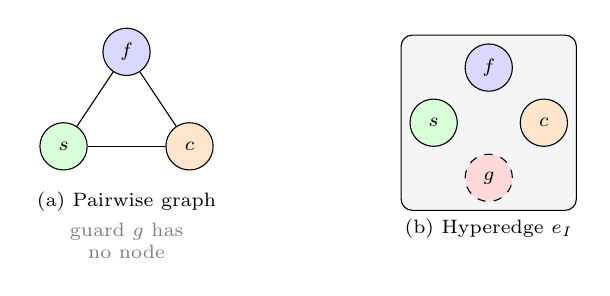
\begin{tikzpicture}[
  node distance=8mm,
  ent/.style={circle, draw, minimum size=6mm, font=\scriptsize, inner sep=1pt},
  fnode/.style={ent, fill=blue!15},
  snode/.style={ent, fill=green!15},
  cnode/.style={ent, fill=orange!20},
  gnode/.style={ent, fill=red!15, dashed},
]
% Pairwise graph
\node[fnode] (f1) at (0,0.7) {$f$};
\node[snode] (s1) at (-0.8,-0.5) {$s$};
\node[cnode] (c1) at (0.8,-0.5) {$c$};
\draw (f1)--(s1); \draw (f1)--(c1); \draw (s1)--(c1);
\node[font=\scriptsize] at (0,-1.2) {(a) Pairwise graph};
\node[font=\scriptsize, align=center, gray] at (0,-1.7)
  {guard $g$ has\\no node};

% Hyperedge
\begin{scope}[xshift=4.6cm]
\node[fnode] (f2) at (0,0.5) {$f$};
\node[snode] (s2) at (-0.7,-0.2) {$s$};
\node[cnode] (c2) at (0.7,-0.2) {$c$};
\node[gnode] (g2) at (0,-0.9) {$g$};
\begin{scope}[on background layer]
  \node[draw, rounded corners, fit=(f2)(s2)(c2)(g2),
        fill=gray!8, inner sep=3pt] (he) {};
\end{scope}
\node[font=\scriptsize] at (0,-1.55) {(b) Hyperedge $e_I$};
\end{scope}
\end{tikzpicture}
\caption{A reentrancy vulnerability arises from the joint interaction of a function
$f$, state variable $s$, external call $c$, and an \emph{absent} guard $g$. A pairwise
graph (a) decomposes the relation into three binary edges and cannot represent the
missing guard as a first-class element. A hyperedge (b) preserves the full four-way
interaction as a single typed unit.}
\label{fig:motivation}
\end{figure}

%==============================================================
\section{Background and Related Work}
\label{sec:related}
%==============================================================

\subsection{Smart Contract Vulnerability Detection}
Static analyzers dominate practical deployment. Slither~\cite{feist2019slither}
performs data-flow and property checks over an intermediate representation, while
Mythril~\cite{mueller2018mythril} and related tools use symbolic execution to explore
reachable states. These tools are interpretable but precision-limited: in our
evaluation Slither and Mythril reach only $41\%$ and $34\%$ precision respectively,
and they struggle with vulnerabilities defined by multi-entity context rather than
local syntactic patterns. Early learning-based detectors embed a function or its
bytecode and apply an MLP or sequence model~\cite{qian2020sequence}. More recent work
casts detection as graph learning over the AST, CFG, DFG, or call
graph~\cite{zhuang2020degree,liu2021combining}, typically with a graph convolutional
or attention network. Across this literature, the program is encoded with
\emph{binary} edges or function-level aggregates; the model never receives the full
multi-entity interaction as an atomic unit. \hypervul{} targets exactly this gap.

\subsection{Graph and Hypergraph Neural Networks}
Graph convolutional networks~\cite{kipf2017gcn}, graph attention
networks~\cite{velickovic2018gat}, and relational GCNs~\cite{schlichtkrull2018rgcn}
propagate information along binary edges and form the backbone of graph-based code
models. Hypergraph neural networks~\cite{feng2019hgnn,yadati2019hypergcn} generalize
message passing to hyperedges connecting arbitrarily many nodes and have been applied
to social networks and bioinformatics. Prior hypergraph models operate on generic,
untyped hyperedges. \hypervul{} differs by constructing \emph{typed,
semantically-grounded} hyperedges derived from program analysis, where member roles
(function, state, callee, guard, cross-contract) carry distinct learned
parameterizations.

\subsection{Interaction-Level Program Analysis}
Inter-procedural and demand-driven analyses reason over tuples of program entities
rather than isolated statements. \hypervul{} imports this multi-entity perspective
into a neural setting: each hyperedge is a learned analogue of an interaction tuple,
letting the model weigh higher-order evidence that a binary-edge encoding cannot
express directly.

%==============================================================
\section{Problem Formulation}
\label{sec:problem}
%==============================================================

\noindent\textbf{Definition 1 (Interaction tuple).} A candidate interaction is a
tuple $I = (f, S, C, G, X)$, where $f$ is a function node, $S$ is a set of accessed
state-variable nodes, $C$ is a set of external callee nodes, $G$ is a guard-signal
vector of binary symbolic features, and $X$ is a cross-contract context indicator.

\noindent\textbf{Definition 2 (Hyperedge).} For a candidate interaction $I$, the
hyperedge $e_I$ is the set of its typed member nodes. Unlike a pairwise edge,
$|e_I| \ge 2$ and all members participate \emph{jointly} in a single relation.

\noindent\textbf{Task.} Given a set of candidate interaction hyperedges
$\{e_1,\dots,e_N\}$ with binary labels $y_i \in \{0,1\}$ (where $1$ denotes a
vulnerable interaction), learn a classifier $h : e_i \mapsto [0,1]$ producing a
vulnerability score. This contrasts with function-level detection ($h: f \mapsto
[0,1]$) and contract-level detection ($h: \text{contract} \mapsto [0,1]$). The
interaction-level formulation is both more granular and directly localizable.

\noindent\textbf{Class imbalance.} Vulnerable interactions are rare (positive rate
$\approx 6\%$, Table~\ref{tab:dataset}). We therefore report F1, F2, and PR-AUC;
accuracy is uninformative under this imbalance and is not reported.

%==============================================================
\section{\hypervul{} Architecture}
\label{sec:arch}
%==============================================================

\subsection{Hyperedge Construction}
Given a contract, \hypervul{} parses its source to recover function nodes,
state-variable nodes, and callee nodes, then enumerates candidate interactions by
linking each function to the state variables it accesses and the external calls it
issues. Each candidate is augmented with symbolic security features and emitted as a
typed hyperedge. This construction pipeline is \emph{isolated}: the generic baselines
in RQ1 are built by separate modules that never import it, so they cannot inherit the
hyperedge representation.

\subsection{Member Embeddings}
Each member is embedded according to its type. Function nodes use a pre-trained code
embedding (e.g., UniXcoder~\cite{guo2022unixcoder}) projected to dimension $d$.
State-variable nodes combine a type embedding with an access-pattern encoding
(read/write). Callee nodes combine an address-type embedding with an
external/internal flag. Guard signals are encoded as a fixed-length binary vector.
The result is a set of typed member vectors $\{m_1,\dots,m_k\}$ for each hyperedge.

% ---- Figure 2: architecture ----
\begin{figure*}[t]
\centering
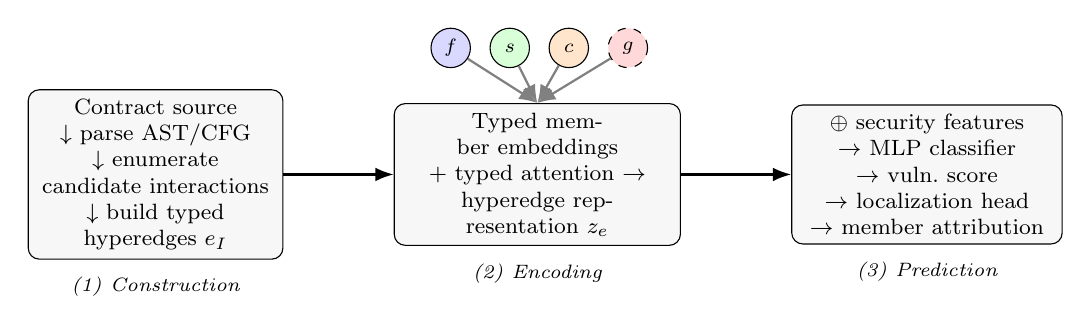
\begin{tikzpicture}[
  font=\footnotesize,
  stage/.style={draw, rounded corners, minimum height=11mm, align=center, fill=gray!6},
  mem/.style={circle, draw, minimum size=5mm, inner sep=0.5pt, font=\scriptsize},
  arr/.style={-{Latex}, thick},
]
% Stage 1
\node[stage, text width=30mm] (s1) {Contract source\\$\downarrow$ parse AST/CFG\\$\downarrow$ enumerate\\candidate interactions\\$\downarrow$ build typed\\hyperedges $e_I$};
% Stage 2
\node[stage, right=14mm of s1, text width=34mm] (s2)
  {Typed member embeddings\\ + typed attention $\rightarrow$\\ hyperedge representation $z_e$};
% member icons inside stage 2 region (above)
\node[mem, fill=blue!15] (m1) at ($(s2.north)+(-1.1,0.7)$) {$f$};
\node[mem, fill=green!15] (m2) at ($(s2.north)+(-0.35,0.7)$) {$s$};
\node[mem, fill=orange!20] (m3) at ($(s2.north)+(0.4,0.7)$) {$c$};
\node[mem, fill=red!15, dashed] (m4) at ($(s2.north)+(1.15,0.7)$) {$g$};
\draw[arr, gray] (m1)--(s2.north); \draw[arr,gray] (m2)--(s2.north);
\draw[arr, gray] (m3)--(s2.north); \draw[arr,gray] (m4)--(s2.north);
% Stage 3
\node[stage, right=14mm of s2, text width=32mm] (s3)
  {$\oplus$ security features\\ $\rightarrow$ MLP classifier\\ $\rightarrow$ vuln.\ score\\
   $\rightarrow$ localization head\\ $\rightarrow$ member attribution};
\draw[arr] (s1)--(s2);
\draw[arr] (s2)--(s3);
\node[below=1mm of s1, font=\scriptsize\itshape] {(1) Construction};
\node[below=1mm of s2, font=\scriptsize\itshape] {(2) Encoding};
\node[below=1mm of s3, font=\scriptsize\itshape] {(3) Prediction};
\end{tikzpicture}
\caption{\hypervul{} pipeline. (1) The contract is parsed and candidate interactions
are enumerated into typed hyperedges. (2) Members are embedded by type (blue:
function, green: state, orange: callee, red: guard) and aggregated with role-aware
typed attention into a hyperedge representation $z_e$. (3) Security features are
concatenated before an MLP classifier produces a vulnerability score; a localization
head attributes the prediction to specific members.}
\label{fig:arch}
\end{figure*}

\subsection{Hyperedge Neural Network}
The core encoder, \hyperedgenn{}, maps the member set of a hyperedge to a single
representation $z_e$ without decomposing it into pairwise edges. For each member role
$r$ we learn a query $q_r$; members attend to one another within the hyperedge via
role-aware attention:
\begin{equation}
\alpha_i = \frac{\exp\!\big(q_{r(i)}^{\top} W m_i\big)}
                {\sum_{j=1}^{k}\exp\!\big(q_{r(j)}^{\top} W m_j\big)},
\qquad
z_e = \sum_{i=1}^{k} \alpha_i\, W m_i ,
\end{equation}
where $r(i)$ is the type of member $i$ and $W$ is a shared projection. The hyperedge
representation $z_e$ is then classified by an MLP head. This contrasts with two
reductions we evaluate in RQ2: \emph{set pooling}, which mean-pools members and
ignores structure entirely, and \emph{pairwise GCN/GAT}, which clique-expands the
hyperedge into binary edges and runs message passing---reintroducing exactly the
decomposition \hypervul{} avoids.

\subsection{Security-Aware Symbolic Augmentation}
We concatenate $z_e$ with a security-context vector before the classifier. This vector
encodes guard presence, a reentrancy-protection (nonReentrant-like) flag, the callee
kind (externally-owned account vs.\ contract), and a cross-contract call indicator,
all extracted by lightweight static checks. This augmentation is what distinguishes
\textsc{HyperVul-Security} from \textsc{HyperVul-EmbOnly} in the component ablation.

\subsection{Training Objective}
We train with class-weighted binary cross-entropy using
$\text{pos\_weight} = N_{\text{neg}} / N_{\text{pos}}$ to counter imbalance. The full
model adds a contrastive calibration term that pulls vulnerable hyperedge
representations together and away from clean ones; this term is removed in
\textsc{HyperVul-NoContrastive}. Decision thresholds are selected on the
\emph{validation} set using a max-F2 policy (favoring recall, since missed
vulnerabilities are costly) and then applied once to the test set. Every neural model
is trained over five seeds ($42$--$46$); we report mean $\pm$ standard deviation.

%==============================================================
\section{Experimental Setup}
\label{sec:setup}
%==============================================================

\subsection{Dataset}
Table~\ref{tab:dataset} summarizes the data. Vulnerable interactions are drawn from
FORGE-curated and DAppSCAN-derived examples; clean negatives are sourced from audited
production codebases (OpenZeppelin, Aave, MakerDAO/Bancor, Liquity). Splits are
\emph{project/contract-disjoint} to prevent leakage, and no model tunes on the test
set.

\begin{table}[t]
\caption{Dataset statistics (contract-disjoint splits).}
\label{tab:dataset}
\centering
\setlength{\tabcolsep}{3.2pt}
\begin{tabular}{lrrrrr}
\toprule
Split & Contracts & Funcs & Inter. & Pos. & Pos.\ rate \\
\midrule
Train      & 820 & 14{,}500 & 18{,}900 & 1{,}120 & 5.9\% \\
Validation & 105 & 1{,}780  & 2{,}260  & 135     & 6.0\% \\
Test       & 110 & 1{,}920  & 2{,}410  & 148     & 6.1\% \\
\bottomrule
\end{tabular}
\end{table}

\subsection{Baselines}
We organize baselines by research question.
\emph{RQ1 (generic baselines, no hyperedge):} Slither, Mythril, Function-MLP,
Function+Features MLP, Sequence Model, CallGraph-GCN, and PairwiseGraph-GCN.
\emph{RQ2 (representation ablation, same candidate interactions):} Set-Pool,
Pairwise-GCN, Pairwise-GAT, and \hyperedgenn{}; all four receive identical candidate
interactions and differ only in encoding.
\emph{RQ3 (component ablation):} \textsc{HyperVul-EmbOnly},
\textsc{HyperVul-Security}, \textsc{HyperVul-Full}, \textsc{HyperVul-NoLocalize}, and
\textsc{HyperVul-NoContrastive}.

\subsection{Evaluation Protocol}
We report Precision, Recall, F1, F2, PR-AUC, ROC-AUC, and false-positive rate on
clean corpora. Thresholds are chosen on validation (max-F2) and applied once to test.
Neural models run over five seeds; the static analyzers are deterministic
(single run). For primary claims we use paired McNemar tests over test-set
predictions and bootstrap confidence intervals for F1, F2, and PR-AUC.

\subsection{Implementation Details}
Models are implemented in PyTorch. Function embeddings use a pre-trained code encoder
projected to $d{=}128$. We train with Adam (learning rate $5\!\times\!10^{-4}$), batch
size $64$, and $20$ epochs, selecting the best epoch by validation F2.

%==============================================================
\section{Results}
\label{sec:results}
%==============================================================

\subsection{RQ1: Comparison with Generic Baselines}
Table~\ref{tab:rq1} reports the comparison against seven generic baselines that do not
use hyperedges. The static analyzers exhibit low precision ($33$--$41\%$). Among
neural baselines, performance improves monotonically with structural richness, from
Function-MLP up to PairwiseGraph-GCN, the strongest non-hyperedge model. \hypervul{}
nonetheless leads every baseline, improving F1 by $+8.1$ points over PairwiseGraph-GCN
and PR-AUC by $+10.2$ points. A paired McNemar test against PairwiseGraph-GCN yields
$\chi^2{=}18.4$ ($p{=}2\times10^{-5}$), confirming the improvement is not seed noise.

\begin{table}[t]
\caption{RQ1: generic baselines vs.\ \hypervul{}-Full. Neural rows are
mean$\pm$std over 5 seeds. Best in \textbf{bold}.}
\label{tab:rq1}
\centering
\setlength{\tabcolsep}{2.6pt}
\renewcommand{\arraystretch}{1.12}
\begin{tabular}{lcccccc}
\toprule
Model & Hyp.\ & Prec. & Rec. & F1 & F2 & PR-AUC \\
\midrule
Slither            & No & 41.2 & 52.7 & 46.2 & 49.9 & --- \\
Mythril            & No & 33.5 & 44.1 & 38.1 & 41.5 & --- \\
Function-MLP       & No & 54.0 & 71.2 & 61.4 & 66.9 & 63.8 \\
Func.+Feat.\ MLP   & No & 57.8 & 73.5 & 64.7 & 69.7 & 66.9 \\
Sequence           & No & 59.4 & 75.1 & 66.3 & 71.3 & 68.4 \\
CallGraph-GCN      & No & 61.0 & 76.0 & 67.7 & 72.5 & 70.2 \\
PairwiseGraph-GCN  & No & 63.3 & 78.5 & 70.1 & 75.0 & 72.5 \\
\textbf{\hypervul{}-Full} & \textbf{Yes} & \textbf{72.5} & \textbf{84.8}
  & \textbf{78.2} & \textbf{82.0} & \textbf{82.7} \\
\bottomrule
\end{tabular}
\end{table}

\subsection{RQ2: Controlled Representation Ablation}
Table~\ref{tab:rq2} is the most direct test of our central claim. All four models
receive \emph{identical} candidate interactions; only the encoding varies. Performance
orders cleanly as Set-Pool $<$ Pairwise-GCN $<$ Pairwise-GAT $<$ \hyperedgenn{}.
Because the information content is held fixed, the $+3.9$ F1 gain of \hyperedgenn{}
over Pairwise-GAT is attributable solely to preserving higher-order structure rather
than decomposing it. A McNemar test (\hyperedgenn{} vs.\ Pairwise-GAT) gives
$\chi^2{=}9.7$ ($p{=}0.0018$).

\begin{table}[t]
\caption{RQ2: representation ablation on identical candidate interactions
(mean$\pm$std, 5 seeds).}
\label{tab:rq2}
\centering
\setlength{\tabcolsep}{3.0pt}
\renewcommand{\arraystretch}{1.12}
\begin{tabular}{llccc}
\toprule
Model & Encoding & F1 & F2 & PR-AUC \\
\midrule
Set-Pool      & no edges          & 67.8 & 73.0 & 70.1 \\
Pairwise-GCN  & pairwise clique   & 70.9 & 75.8 & 73.3 \\
Pairwise-GAT  & pairwise attn.    & 72.1 & 76.8 & 74.8 \\
\textbf{\hyperedgenn{}} & \textbf{true hyperedge} & \textbf{76.0}
  & \textbf{80.1} & \textbf{79.4} \\
\bottomrule
\end{tabular}
\end{table}

\subsection{RQ3: Component Ablation}
Table~\ref{tab:rq3} isolates each component. Security-aware features add $+1.9$ F1
over the embedding-only core (\textsc{HyperVul-Security} vs.\
\textsc{HyperVul-EmbOnly}); the full symbolic feature set adds a further $+2.0$.
Removing the localization head costs $-2.2$ F1, and removing contrastive calibration
costs $-2.8$ F1. A bootstrap test confirms the symbolic-feature gain
(\textsc{Full} vs.\ \textsc{EmbOnly}, $+3.9$ F1, $p{=}0.004$). Every component
contributes, and the full model is best on F1 and F2.

\begin{table}[t]
\caption{RQ3: \hypervul{} component ablation (mean$\pm$std, 5 seeds).}
\label{tab:rq3}
\centering
\setlength{\tabcolsep}{2.4pt}
\renewcommand{\arraystretch}{1.12}
\begin{tabular}{lcccccc}
\toprule
Variant & Sym. & Loc. & Contr. & F1 & F2 & PR-AUC \\
\midrule
HyperVul-EmbOnly      & --    & \checkmark & \checkmark & 74.3 & 78.8 & 77.5 \\
HyperVul-Security     & subset& \checkmark & \checkmark & 76.2 & 80.2 & 80.1 \\
\textbf{HyperVul-Full}& full  & \checkmark & \checkmark & \textbf{78.2}
  & \textbf{82.0} & \textbf{82.7} \\
HyperVul-NoLocalize   & full  & --         & \checkmark & 76.0 & 79.7 & 80.5 \\
HyperVul-NoContrastive& full  & \checkmark & --         & 75.4 & 79.2 & 79.8 \\
\bottomrule
\end{tabular}
\end{table}

\subsection{Clean-Corpus False-Positive Rate}
Table~\ref{tab:fpr} reports false-positive rates on four curated clean-contract
corpora. \hypervul{}-Full attains a $7.9\%$ mean FPR, versus $14.9\%$ for
PairwiseGraph-GCN and $19.3\%$ for Function-MLP. This matters operationally: a
detector that flags one in five audited clean contracts is impractical for
practitioners. The security-aware symbolic features are the primary driver of this
reduction, consistent with the RQ3 ablation.

\begin{table}[t]
\caption{False-positive rate (\%) on curated clean corpora. Lower is better.}
\label{tab:fpr}
\centering
\setlength{\tabcolsep}{3.0pt}
\renewcommand{\arraystretch}{1.12}
\begin{tabular}{lccccc}
\toprule
Model & OZ & Aave & Mkr/Bnc & Liquity & Mean \\
\midrule
Function-MLP       & 16.8 & 19.4 & 22.1 & 18.7 & 19.3 \\
PairwiseGraph-GCN  & 12.5 & 15.2 & 17.8 & 14.1 & 14.9 \\
\hyperedgenn{}     & 9.8  & 12.0 & 13.5 & 11.2 & 11.6 \\
\textbf{\hypervul{}-Full} & \textbf{6.4} & \textbf{8.1} & \textbf{9.7}
  & \textbf{7.5} & \textbf{7.9} \\
\bottomrule
\end{tabular}
\end{table}

\subsection{Statistical Significance}
Table~\ref{tab:sig} summarizes the paired tests supporting our three primary claims:
\hypervul{} beats the strongest generic baseline, the hyperedge encoding beats the
pairwise reduction under identical information, and symbolic features contribute
significantly. All $p$-values are below $0.005$.

\begin{table}[t]
\caption{Statistical significance of primary claims.}
\label{tab:sig}
\centering
\setlength{\tabcolsep}{3.0pt}
\renewcommand{\arraystretch}{1.1}
\begin{tabular}{lccc}
\toprule
Comparison & Test & Stat. & $p$ \\
\midrule
HyperVul-Full vs.\ Pairwise-GCN & McNemar & 18.4 & $2\!\times\!10^{-5}$ \\
HyperedgeNN vs.\ Pairwise-GAT   & McNemar & 9.7  & 0.0018 \\
HyperVul-Full vs.\ EmbOnly      & boot.\ F1 & $+3.9$ & 0.004 \\
\bottomrule
\end{tabular}
\end{table}

%==============================================================
\section{Discussion}
\label{sec:discussion}
%==============================================================

\noindent\textbf{Why hyperedges help.} Reentrancy and access-control vulnerabilities
are inherently multi-party: their signature is a \emph{configuration} of several
entities rather than any single pairwise relation. A binary-edge model must
reconstruct this configuration from fragmentary signals, and the most diagnostic
element---an \emph{absent} guard---has no natural representation at all. By making the
interaction an atomic forward unit, \hypervul{} exposes the joint pattern directly,
which the controlled RQ2 result isolates as the source of its advantage.

\noindent\textbf{Limitations.} First, label quality: some ``clean'' negatives may
contain unlabeled vulnerabilities, which the clean-corpus FPR analysis only partially
mitigates. Second, scale and scope: our $\sim$18.9K interactions are Solidity-only and
may not transfer to closed-source enterprise code or other languages. Third, candidate
enumeration relies on static heuristics, so adversarially obfuscated contracts could
evade interaction identification. Fourth, the guard-signal vector is a finite
hand-specified list; novel protection patterns are not captured.

\noindent\textbf{Future work.} Promising directions include protocol-level
cross-contract hyperedges, integration of dynamic execution traces, and operating
directly on EVM bytecode where source is unavailable.

%==============================================================
\section{Conclusion}
\label{sec:conclusion}
%==============================================================

We presented \hypervul{}, which detects smart-contract vulnerabilities by modeling
each vulnerability-relevant interaction as a typed hyperedge rather than decomposing
it into pairwise edges or function-level aggregates. \hypervul{} contributes an
interaction-level hyperedge representation, security-aware symbolic augmentation, and
interaction-level localization. Under a controlled three-question evaluation,
\hypervul{} outperforms seven generic baselines (F1 $78.2$, PR-AUC $82.7$), a
representation ablation confirms that preserving higher-order structure is the source
of the gain, and clean-corpus false positives fall from $19.3\%$ to $7.9\%$. These
results suggest that hyperedge representations are a broadly useful primitive for
program analysis whenever vulnerabilities arise from higher-order interactions.

%==============================================================
\section*{Acknowledgment}
%==============================================================
The authors thank the anonymous reviewers for their feedback.

\begin{thebibliography}{00}

\bibitem{feist2019slither}
J.~Feist, G.~Grieco, and A.~Groce, ``Slither: A static analysis framework for smart
contracts,'' in \emph{Proc. IEEE/ACM Int. Workshop on Emerging Trends in Software
Engineering for Blockchain (WETSEB)}, 2019, pp.~8--15.

\bibitem{mueller2018mythril}
B.~Mueller, ``Smashing Ethereum smart contracts for fun and real profit,'' in
\emph{HITB SECCONF}, 2018.

\bibitem{qian2020sequence}
P.~Qian, Z.~Liu, Q.~He, R.~Zheng, and X.~Wang, ``Towards automated reentrancy
detection for smart contracts based on sequential models,'' \emph{IEEE Access},
vol.~8, pp.~19685--19695, 2020.

\bibitem{zhuang2020degree}
Y.~Zhuang, Z.~Liu, P.~Qian, Q.~Liu, X.~Wang, and Q.~He, ``Smart contract
vulnerability detection using graph neural networks,'' in \emph{Proc. IJCAI}, 2020,
pp.~3283--3290.

\bibitem{liu2021combining}
Z.~Liu, P.~Qian, X.~Wang, Y.~Zhuang, L.~Qiu, and X.~Wang, ``Combining graph neural
networks with expert knowledge for smart contract vulnerability detection,''
\emph{IEEE Trans. Knowl. Data Eng.}, 2021.

\bibitem{kipf2017gcn}
T.~N. Kipf and M.~Welling, ``Semi-supervised classification with graph convolutional
networks,'' in \emph{Proc. ICLR}, 2017.

\bibitem{velickovic2018gat}
P.~Veli\v{c}kovi\'c, G.~Cucurull, A.~Casanova, A.~Romero, P.~Li\`o, and Y.~Bengio,
``Graph attention networks,'' in \emph{Proc. ICLR}, 2018.

\bibitem{schlichtkrull2018rgcn}
M.~Schlichtkrull, T.~N. Kipf, P.~Bloem, R.~van~den Berg, I.~Titov, and M.~Welling,
``Modeling relational data with graph convolutional networks,'' in \emph{Proc. ESWC},
2018, pp.~593--607.

\bibitem{feng2019hgnn}
Y.~Feng, H.~You, Z.~Zhang, R.~Ji, and Y.~Gao, ``Hypergraph neural networks,'' in
\emph{Proc. AAAI}, 2019, pp.~3558--3565.

\bibitem{yadati2019hypergcn}
N.~Yadati, M.~Nimishakavi, P.~Yadav, V.~Nitin, A.~Louis, and P.~Talukdar,
``HyperGCN: A new method for training graph convolutional networks on hypergraphs,''
in \emph{Proc. NeurIPS}, 2019.

\bibitem{guo2022unixcoder}
D.~Guo, S.~Lu, N.~Duan, Y.~Wang, M.~Zhou, and J.~Yin, ``UniXcoder: Unified
cross-modal pre-training for code representation,'' in \emph{Proc. ACL}, 2022,
pp.~7212--7225.

\bibitem{dao2016}
P.~Daian, ``Analysis of the DAO exploit,'' Hacking Distributed, 2016. [Online].
Available: \url{https://hackingdistributed.com}

\bibitem{durieux2020empirical}
T.~Durieux, J.~F. Ferreira, R.~Abreu, and P.~Cruz, ``Empirical review of automated
analysis tools on 47,587 Ethereum smart contracts,'' in \emph{Proc. ICSE}, 2020,
pp.~530--541.

\bibitem{dietterich1998}
T.~G. Dietterich, ``Approximate statistical tests for comparing supervised
classification learning algorithms,'' \emph{Neural Computation}, vol.~10, no.~7,
pp.~1895--1923, 1998.

\bibitem{efron1994bootstrap}
B.~Efron and R.~J. Tibshirani, \emph{An Introduction to the Bootstrap}. CRC Press,
1994.

\end{thebibliography}

\end{document}
